% Options for packages loaded elsewhere
\PassOptionsToPackage{unicode}{hyperref}
\PassOptionsToPackage{hyphens}{url}
%
\documentclass[
]{article}
\usepackage{amsmath,amssymb}
\usepackage{lmodern}
\usepackage{iftex}
\ifPDFTeX
  \usepackage[T1]{fontenc}
  \usepackage[utf8]{inputenc}
  \usepackage{textcomp} % provide euro and other symbols
\else % if luatex or xetex
  \usepackage{unicode-math}
  \defaultfontfeatures{Scale=MatchLowercase}
  \defaultfontfeatures[\rmfamily]{Ligatures=TeX,Scale=1}
\fi
% Use upquote if available, for straight quotes in verbatim environments
\IfFileExists{upquote.sty}{\usepackage{upquote}}{}
\IfFileExists{microtype.sty}{% use microtype if available
  \usepackage[]{microtype}
  \UseMicrotypeSet[protrusion]{basicmath} % disable protrusion for tt fonts
}{}
\makeatletter
\@ifundefined{KOMAClassName}{% if non-KOMA class
  \IfFileExists{parskip.sty}{%
    \usepackage{parskip}
  }{% else
    \setlength{\parindent}{0pt}
    \setlength{\parskip}{6pt plus 2pt minus 1pt}}
}{% if KOMA class
  \KOMAoptions{parskip=half}}
\makeatother
\usepackage{xcolor}
\IfFileExists{xurl.sty}{\usepackage{xurl}}{} % add URL line breaks if available
\IfFileExists{bookmark.sty}{\usepackage{bookmark}}{\usepackage{hyperref}}
\hypersetup{
  pdftitle={Exploring the effect of conversion on the distribution of inflectional suffixes: a multivariate corpus study},
  hidelinks,
  pdfcreator={LaTeX via pandoc}}
\urlstyle{same} % disable monospaced font for URLs
\usepackage[margin=1in]{geometry}
\usepackage{longtable,booktabs,array}
\usepackage{calc} % for calculating minipage widths
% Correct order of tables after \paragraph or \subparagraph
\usepackage{etoolbox}
\makeatletter
\patchcmd\longtable{\par}{\if@noskipsec\mbox{}\fi\par}{}{}
\makeatother
% Allow footnotes in longtable head/foot
\IfFileExists{footnotehyper.sty}{\usepackage{footnotehyper}}{\usepackage{footnote}}
\makesavenoteenv{longtable}
\usepackage{graphicx}
\makeatletter
\def\maxwidth{\ifdim\Gin@nat@width>\linewidth\linewidth\else\Gin@nat@width\fi}
\def\maxheight{\ifdim\Gin@nat@height>\textheight\textheight\else\Gin@nat@height\fi}
\makeatother
% Scale images if necessary, so that they will not overflow the page
% margins by default, and it is still possible to overwrite the defaults
% using explicit options in \includegraphics[width, height, ...]{}
\setkeys{Gin}{width=\maxwidth,height=\maxheight,keepaspectratio}
% Set default figure placement to htbp
\makeatletter
\def\fps@figure{htbp}
\makeatother
\setlength{\emergencystretch}{3em} % prevent overfull lines
\providecommand{\tightlist}{%
  \setlength{\itemsep}{0pt}\setlength{\parskip}{0pt}}
\setcounter{secnumdepth}{5}
\newlength{\cslhangindent}
\setlength{\cslhangindent}{1.5em}
\newlength{\csllabelwidth}
\setlength{\csllabelwidth}{3em}
\newlength{\cslentryspacingunit} % times entry-spacing
\setlength{\cslentryspacingunit}{\parskip}
\newenvironment{CSLReferences}[2] % #1 hanging-ident, #2 entry spacing
 {% don't indent paragraphs
  \setlength{\parindent}{0pt}
  % turn on hanging indent if param 1 is 1
  \ifodd #1
  \let\oldpar\par
  \def\par{\hangindent=\cslhangindent\oldpar}
  \fi
  % set entry spacing
  \setlength{\parskip}{#2\cslentryspacingunit}
 }%
 {}
\usepackage{calc}
\newcommand{\CSLBlock}[1]{#1\hfill\break}
\newcommand{\CSLLeftMargin}[1]{\parbox[t]{\csllabelwidth}{#1}}
\newcommand{\CSLRightInline}[1]{\parbox[t]{\linewidth - \csllabelwidth}{#1}\break}
\newcommand{\CSLIndent}[1]{\hspace{\cslhangindent}#1}
\usepackage{caption}
\usepackage{subcaption}
\ifLuaTeX
  \usepackage{selnolig}  % disable illegal ligatures
\fi

\title{Exploring the effect of conversion on the distribution of
inflectional suffixes: a multivariate corpus study}
\author{Alexander Rauhut\\
Institut für Englische Philologie\\
Freie Universität Berlin}
\date{2021-07-15}

\begin{document}
\maketitle

{
\setcounter{tocdepth}{2}
\tableofcontents
}
\newpage

\hypertarget{introduction}{%
\section{Introduction}\label{introduction}}

The English language makes it easy to verb a noun. Conversion is a
remarkably productive word formation process in analytic languages. Yet
little quantitative research has been presented on the topic. This study
will focus on word class ambiguity and explore the effect on the
distribution of inflections. I will attempt to show that the probability
of inflectional suffixes is affected by the relative frequency of
nominal versus verbal uses, textual specificity, as well as lexical and
contextual boundedness. Forms that are similarly associated to both
categories exist in a potential ``uncanny valley'', and it will be
argued that there is a noticeably different distribution of inflectional
suffixes for those forms. These differences might point to systemic
tendencies or even restrictions that, among other reasons, could be
caused by a more general tendency to avoid ambiguity.

Ambiguity is pervasive in language. In fact, the term itself is
ambiguous and there is a plethora of types of ambiguity that have been
recognized by linguists. On the structural level of English, ambiguities
can be roughly categorized into two broad categories of syntactic, and
lexical ambiguities. Lexical ambiguity most frequently occurs when there
is polysemy or homonymy that may lead to conflicting interpretations.
Syntactic ambiguity arises when there are multiple parses for the same
syntactic pattern. This can itself be directly or indirectly caused by
some form of lexical ambiguity. Word class ambiguity is a type of
ambiguity that is not so commonly in focus. There is little potential
for misinterpreting conversion or accidentally assuming conversion. Most
lexemes that are commonly categorized as belonging to one of the open
word classes are word class ambiguous only outside of a communicative
context. Word class information and other grammatical and distributional
information is stored in memory as part of the information about the
lexeme, so this ambiguity is inherently a matter of degree. Lexical
items are more or less strongly entrenched. How word class ambiguous a
lexeme is also depends on the distributional make-up and semantic
properties. The aim of this study is not to identify and ag actual cases
of ambiguity that are caused by conversion, but rather large scale
effects and tendencies on the composition of the lexical system. The
underlying question is why a language like English allows to readily use
a lexical item as either noun or verb even though there is little
morphological marking in English.

The emergence of lexical clusters, including polysemes, homonyms or
multi-word expressions is conditioned by frequency. In an exemplar-based
model, word classes themselves are expected to emerge through
categorizing and clustering of contiguous experiences,
e.g.~(co-)occurrence patterns. Various studies have provided evidence
for frequency and clustering effects (for a review, cf.
\protect\hyperlink{ref-diessel16}{Diessel 2016}). Conversely, the lack
of distinctiveness between (co-)occurrence patterns is expected to cause
fuzzier, generally less well-entrenched categories. If conversion
becomes too frequent, the clustering of occurrences per lexeme and the
learned associations to the word classes would be weakened for the
affected items.

In section \ref{avoid} and \ref{proc}, I will outline the phenomenon and
review experimental Phonetics and Neurolinguistics literature on the
effects of ambiguity and ambiguity avoidance, and discuss some arguments
on the role and limits of ambiguity. Section \ref{conv_measure} is
concerned with the conceptualization and operationalization of
conversion, and section \ref{meth} will provide an overview over the
metrics used in this study. Subsequently, in section \ref{analys}, I
will present a series of GAMLSS models (Generalized Additive Models for
Location, Scale and Shape,
\protect\hyperlink{ref-stasinopoulos18}{Stasinopoulos, Rigby \& Bastiani
2018}; \protect\hyperlink{ref-gamlss}{Rigby \& Stasinopoulos 2005}) that
attempt to model the influence of verb-noun or noun-verb conversion on
the distribution of \emph{-s} and \emph{-ed} suffixation while
controlling for textual dispersion, regularity of occurrence and
contextual flexibility. In Section \ref{disc}, the results will be
discussed in light of considerations from previous sections. Section
\ref{conc} concludes the findings and provides suggestions for
improvements in methodology. \footnote{The data was preprocessed using
  the \emph{Corpus Workbench} (\protect\hyperlink{ref-cwb}{Evert \&
  Hardie 2011}), all ags were coded in \emph{R} 4.1.0
  (\protect\hyperlink{ref-R_base}{R Core Team 2021};
  \protect\hyperlink{ref-data.table}{Dowle \& Srinivasan 2021}), figures
  were created with \emph{ggplot2}
  (\protect\hyperlink{ref-ggplot}{Wickham 2016}).}

\hypertarget{word-class-ambiguity}{%
\section{Word class ambiguity}\label{word-class-ambiguity}}

\hypertarget{avoid}{%
\subsection{Potential functions of ambiguity}\label{avoid}}

Wasow (\protect\hyperlink{ref-wasow15}{2015}) provides an overview of
different types of ambiguities. Among other types, the author points out
that word order freezing might be seen as ambiguity avoidance. The
ambiguity that is hypothesized to be avoided here is understood to be
concerning syntactic relations. However, word order freezing also avoids
word class ambiguity in a mostly inflection-free grammar. German has a
rather free word order, but the finite verb is also frozen in second
position, which equally avoids word class ambiguity, especially
considering German bare infinitives are a common means of
nominalization. Wasow (\protect\hyperlink{ref-wasow15}{2015}) finally
concludes that ambiguity avoidance has not been shown to be as common as
expected considering the pervasiveness of ambiguities in language.

Phonetic changes are often the trigger for the emergence of homonymy and
some types of syntactic ambiguity, mostly those caused by syncretism via
morphological reduction. Evidently, those ambiguities are often not
immediately resolved or compensated for in an obvious way. Past research
has tried to explain the existence and even necessity of ambiguity in
natural languages. There seem to be good reasons for the pervasiveness
of ambiguity, and good reasons for a language to keep ambiguity at a
minimum. In both cases, ease of processing and ease of production
represent convincing candidates (cf.
\protect\hyperlink{ref-piantadosi_et_al12}{Piantadosi, Tily \& Gibson
2012}; \protect\hyperlink{ref-tomaschek_et_al_18}{Tomaschek et al.
2018}). They are also competing motivations potentially balancing the
amount of ambiguity in a language. Piantadosi, Tily \& Gibson
(\protect\hyperlink{ref-piantadosi_et_al12}{2012}) argue that some
degree of ambiguity is required in an efficient communicative system.
More recently, Trott \& Bergen
(\protect\hyperlink{ref-trott+bergen20}{2020}) argued that, based on
simulation, linguistic forms are expected to show a certain degree of
ambiguity in order to provide an efficient system. Their simulations
suggest that ambiguity caused by homophony is more common in natural
languages than expected, despite the processing and efficiency
advantages. Furthermore, homophones were shown to be smoothed out in
lexically neighboring areas.

Given the plethora of contextual information in any given communicative
situation, a different reason for the perceived pervasiveness of
ambiguity is that there is usually enough context to disambiguate.
Studies like Plag, Homann \& Kunter
(\protect\hyperlink{ref-plag17}{2017}) on word-final \emph{-s} call into
question how common perfect homophony actually is. The study found
significant length differences, and hypothesizes that subtle phonetic
differences are learned and contribute to the lexical representation of
words in memory. Yung Song et al.
(\protect\hyperlink{ref-song_et_al13}{2013}) did not find any such
effect, albeit on a more lexically restricted study. Systematic phonetic
differences potentially contribute to disambiguation, rendering
ambiguity through homonymy more of a surface phenomenon. In a more
recent study, Tomaschek et al.
(\protect\hyperlink{ref-tomaschek_et_al21}{2021}) show that length of
final \emph{-s} can be modeled as having a discriminatory function
depending on the lexical and phonological context. In other words, the
duration was found to decrease with increasing contextual ambiguity.
``Energy is not invested in a signal that creates confusion instead of
clarity.'' (\protect\hyperlink{ref-tomaschek_et_al21}{Tomaschek et al.
2021: 154}) This points to some degree of ambiguity sensitivity, even
though it is not entirely clear what it means for ambiguity avoidance.
Assuming the inverse of this observation is equally the case, namely
that more energy is invested in a signal that creates clarity, an
interesting analogical hypothesis could be formulated that word class
ambiguous lexemes are potentially reinforced by additional
morpho-syntactic marking even though they are not necessarily likely to
produce ambiguity. In that case, redundancies in marking are to be
expected.

\hypertarget{proc}{%
\subsection{Word class ambiguity and processing}\label{proc}}

In neurolinguistic experiments it has been observed that word class
ambiguity leads to a significantly longer processing time of word class
ambiguous items (\protect\hyperlink{ref-federmeier_et_al00}{Federmeier
et al. 2000}; \protect\hyperlink{ref-lee+federmeier08}{Lee \& Federmeier
2008}). This correlates with the activation of separate regions in
memory for both nominal and verbal representations of the item.
Interestingly, these effects are present even when word class membership
is clear from the context, although those findings have been somewhat
relativized by Lee \& Federmeier (\protect\hyperlink{ref-lee06}{2006}),
where it is argued that other types of semantic ambiguity are also
common in many of the word class ambiguous items, which might cause part
of the effect. Nevertheless, the idea that syntactical context that is
sufficient to disambiguate may still not be enough to optimize
processing time falls in line with the hypothesized need for redundancy
mentioned above. In contrast to the increased difficulty in processing,
and in accordance with the idea of competing motivations, Bultena,
Dijkstra \& Hell (\protect\hyperlink{ref-bultena_et_al13}{2013})
describe a facilitory effect of word class ambiguity for learners.

In order to investigate how word class ambiguity affects the
distribution of the available inflectional markers, the next section
will focus on the frequency distribution of word class per lexical item
in a corpus.

\hypertarget{conv_measure}{%
\subsection{Word class ambiguity in corpora}\label{conv_measure}}

The potential for conversions and word class ambiguity varies from
lexeme to lexeme. Conversion as word formation can be spontaneous or
lexicalized, showing different degrees of conventualization. It can be
assumed that there is a cline allowing for all degrees of lexicalization
and conventionalization from polysemes up to fully fledged homonymy with
varying degrees of lexical association between the nominal and lexical
counterparts.

\begin{enumerate}
\def\labelenumi{(\arabic{enumi})}
\tightlist
\item
  spontaneous: streisanded (twitter hashtag\footnote{\url{https://twitter.com/hashtag/streisanded}})
\item
  lexicalized: a build, to build
\item
  partial homonymy: a form, to form
\item
  full homonymy: a bank, to bank
\end{enumerate}

Conversion is a productive process that inevitably produces homophones.
Additionally, noun-verb and verb-noun conversions are doubly homophonous
with inflectional affixes in \emph{-s}.

\begin{figure}[t!]
   \centering
   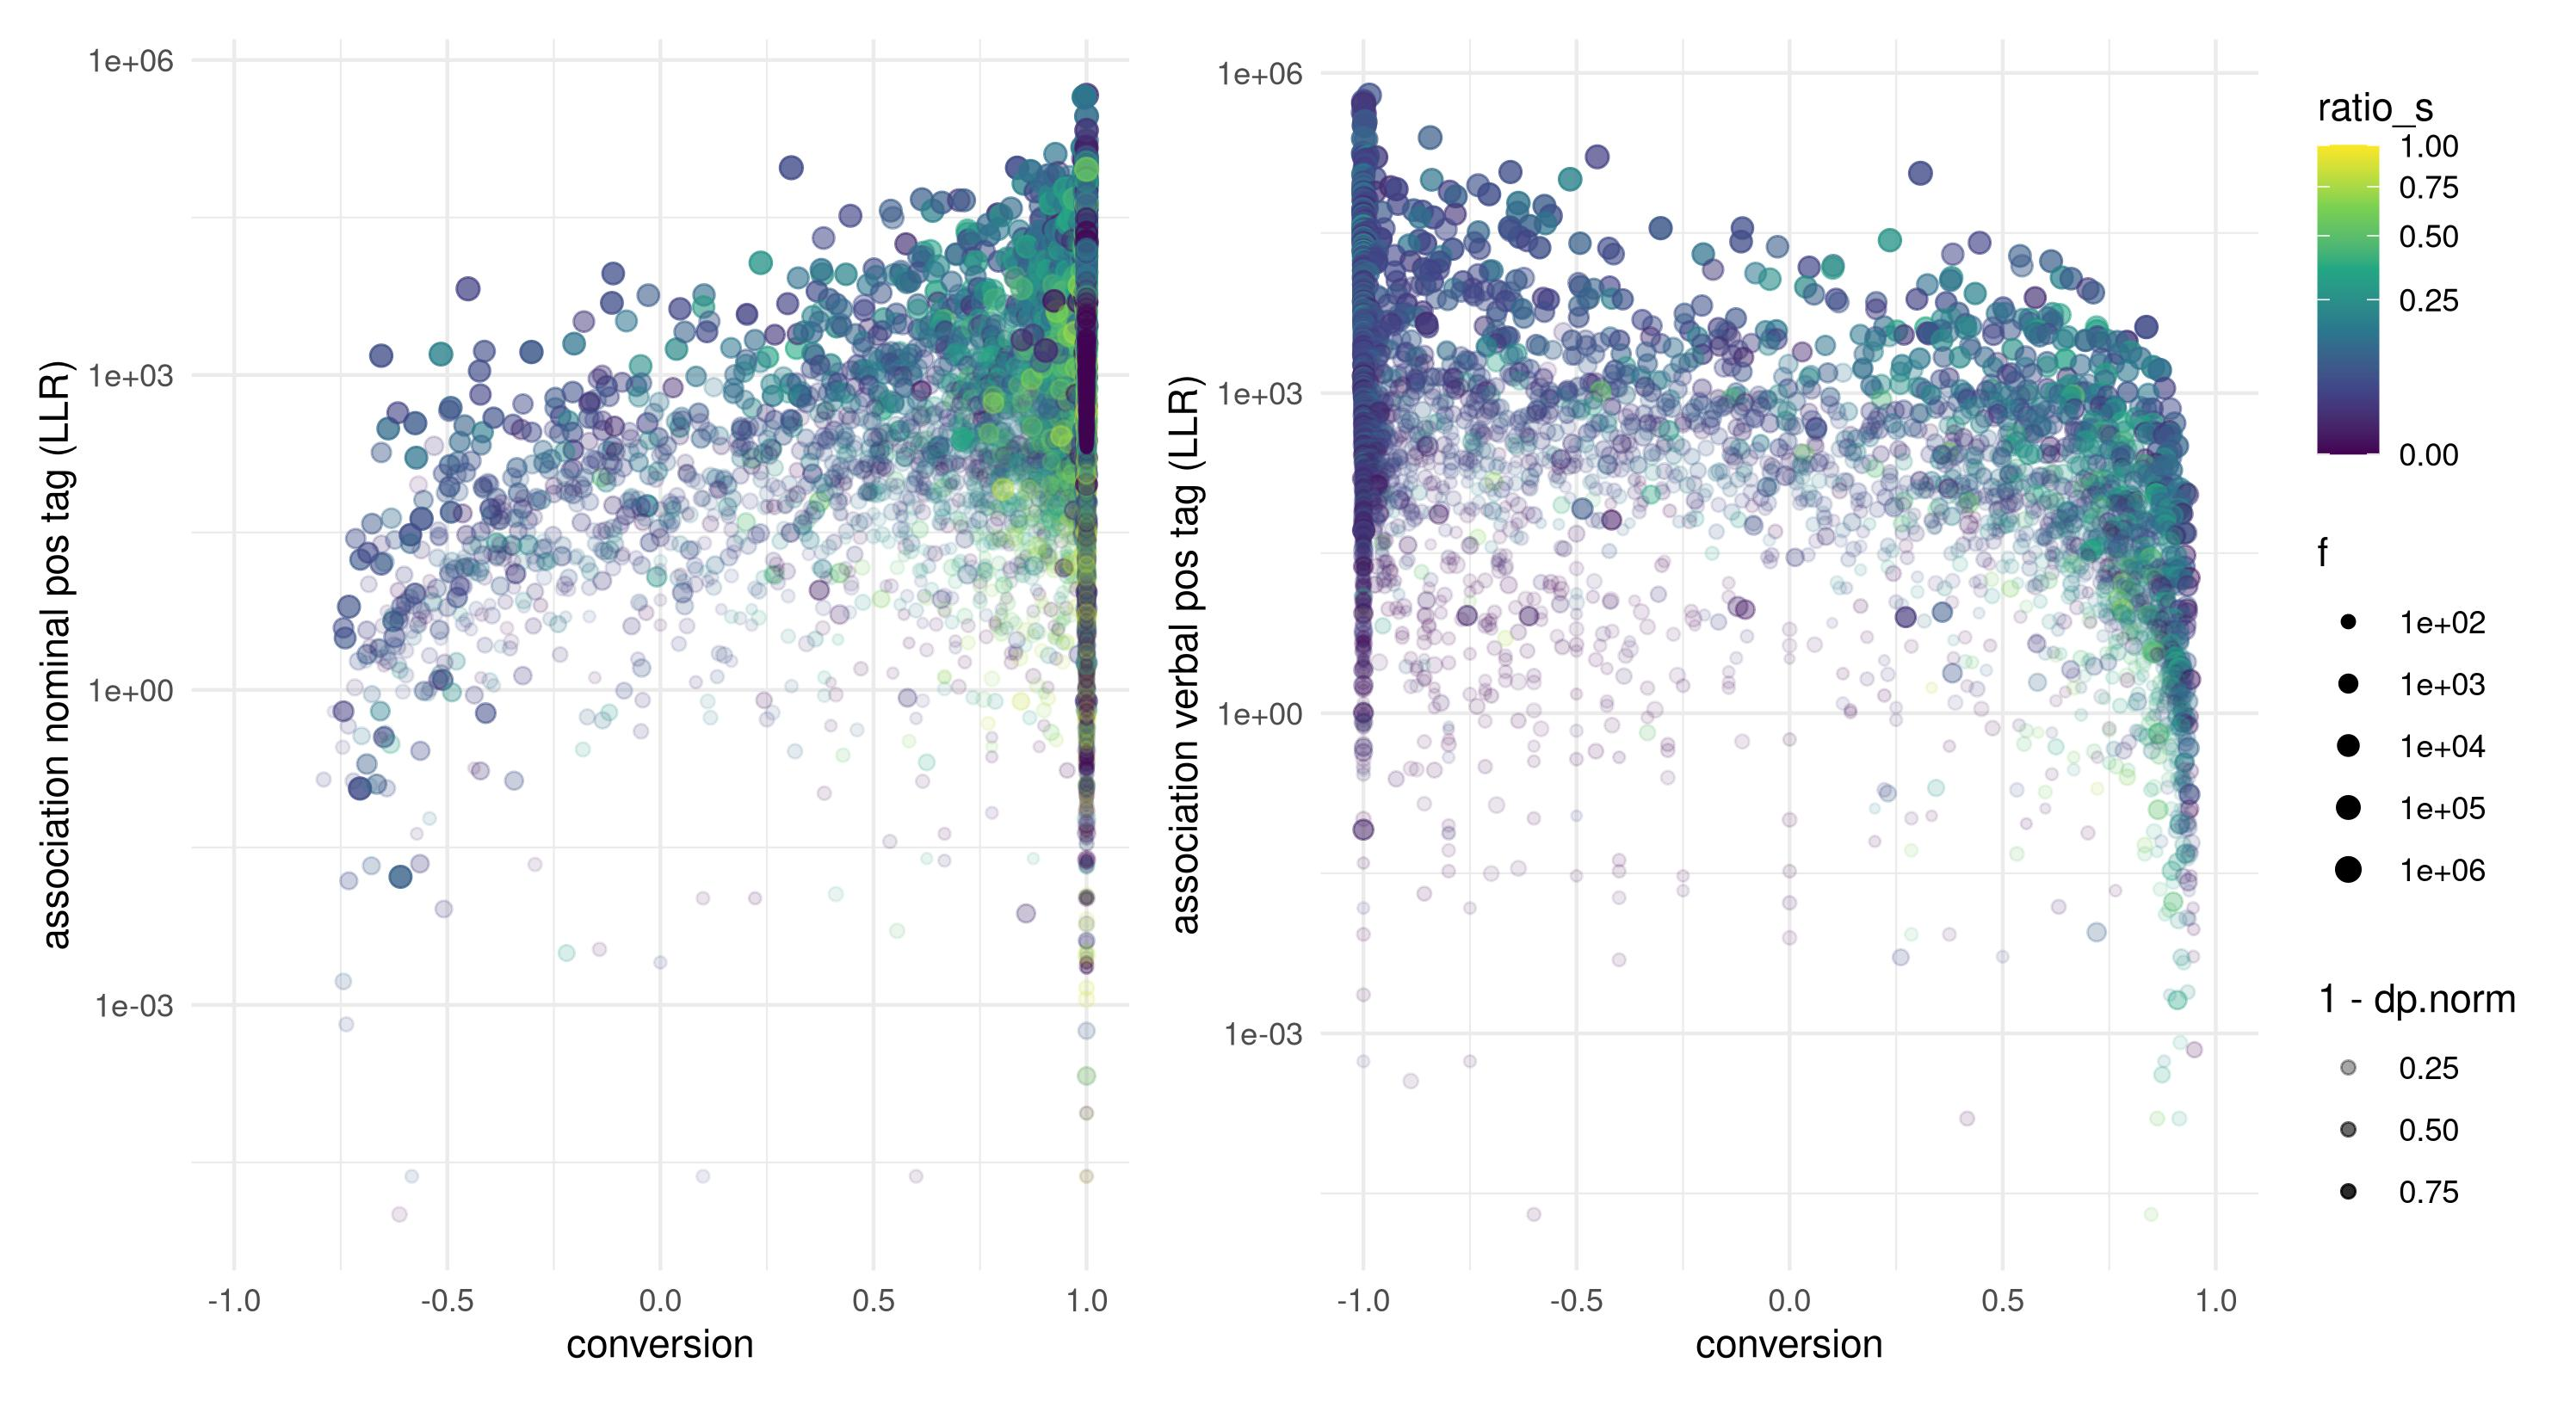
\includegraphics[width=\textwidth]{figures/continuum.jpg}
   \caption{Compound ratio of noun/verb POS tags against attraction}
   \label{continuum}
\end{figure}

In order to express the proportions of nominal and verbal tagging, the
ratio of the less dominant word class to the more dominant word class
was taken per lemma, subtracted 1 for dominantly verbal uses, while 1
was subtracted for dominantly nominal uses. This puts the measure into
the range \([-1, 1]\) with \(-1\) when the item was always tagged as
verb, \(+1\) when it was always tagged as noun and 0 when there was a
perfect balance. Figure \ref{continuum} shows the statistical attraction
(measured by the log-likelihood ratio (cf.
\protect\hyperlink{ref-evert05}{Evert 2005})) to nominal and verbal uses
plotted against the mentioned conversion ratio. Note that the cases with
statistical repulsion are not part of the plot. The measure appears to
connect the two distributions well, resulting in a rather homogenous
continuum across which the attraction to nominal/verbal uses increases
monotonously. The ``uncanny valley'' at around 0 is less densely
populated, which is expected since there should be discretization
effects between the word classes considering afore-mentioned clustering
effects.

\hypertarget{meth}{%
\section{Methodology}\label{meth}}

\hypertarget{disp}{%
\subsection{Textual dispersion}\label{disp}}

In order to measure the textual specificity of lexemes, and account for
lexical items with very specific contextually bound uses, two types of
dispersion are used. The first is the Deviation of Proportions across
corpus parts (\(DP\), \protect\hyperlink{ref-gries08}{Gries 2008}), more
specifically the normalized version (\(DP.norm\),
\protect\hyperlink{ref-lijffijt+gries12}{Lijffijt \& Gries 2012}). As
the basic unit, the individual texts were used based on text ID.
\(DP.norm\) is a corpus-part-based measure bound between 0 and 1. Values
close to 1 indicate a high deviation, therefore a low dispersion. It can
be interpreted as a measure of how evenly tokens are spread over the
corpus parts. Figure \ref{continuum} demonstrates how \(DP\) can be used
for explorative visualization, e.g.~by using it to scale alpha values in
dense overplotted scatterplots.

\(DP\) cannot account for short bursts of occurrences, therefore, Word
Growth Dispersion (\(DWG\))
(\protect\hyperlink{ref-zimmermann20}{Zimmermann 2020}). is used in
addition, which is a whole-corpus measure based on distances between
occurrences. \(DWG\) is a measure of how regularly a token occurs across
an entire corpus occurs across an entire corpus. A geometric
normalization is applied to account for sample size (cf.
\protect\hyperlink{ref-zimmermann20}{Zimmermann 2020}) It is a measure
bound between 0 and 1 with higher values indicating higher dispersion.
Both measures were designed to measure dispersion or commonness of
lexical items as extension to the most commonly used plain frequencies.
The two measures highlight different aspects both conceptually and
empirically (cf. \protect\hyperlink{ref-gries21}{Gries 2021} on using
multiple measures of dispersion and association). Therefore, both
correlate with frequency (\(f\)) of use, even though \(DWG\) does so to
a lesser degree.

Based on observations from previous sections, it is expected that in the
presence of word class ambiguity, a lower context-dependency/lower
clumpiness indirectly leads to higher proportions of inflectional uses
since non-inflectional uses would be more ambiguous and harder to
process. Considering a given dispersion across contexts in which a
lexeme is likely to occur, the existence of avoidance-contexts should
manifest in a penalty to dispersion and make the distribution clumpier.
It is difficult to formally identify avoidance contexts. Lexical and
syntactical correlates of the avoided structure might be avoided as a
side effect, and cause fuzzier overall differences in structure. The
contexts in which ambiguity is avoided/not avoided might be rather
evenly dispersed themselves. This could mask potential clumpiness of
\emph{-s} occurrences adding additional noise. Effects that influence
dispersion might be washed out because of that. Nevertheless, both
measures allow to control for higher than usual frequencies of
observations caused by repetition in rapid succession or concentrated in
few texts.

Both extremely high and extremely low values of \(DWG\) and \(DP.norm\)
suggest special values. Most of the variables used in the model are not
expected to have a monotonic relationship with the proportion of
\emph{-s} occurrences. Very badly dispersed lexemes are overrepresented
in terms of frequency, and an extremely even dispersion suggests uses
typical of function words.

\hypertarget{hapax}{%
\subsection{Fixedness}\label{hapax}}

The ratio of hapaxes (henceforth \(alpha_{1}\)
\protect\hyperlink{ref-evert05}{Evert 2005}: 130) on either side of a
given lexeme was used as a simple measure of how fixed the immediate
lexico-grammatical context is. The term \emph{hapax} is used a bit more
liberally here and refers to types that occur only once in the given
window. For ease of interpretation and in order to capture the fixedness
in smaller units of text, the window was held at 1 token to the left and
right. Preliminary experiments with larger windows were inconclusive, so
the simplest version was used. The left and right contexts were also
kept separate since lumping them together conflates quite different
pieces of information, considering the direction of processing, the
branching structure of English, priming effects etc. For example, a
token that is always preceded by a definite article as a part of a name
scores an extremely low \(alpha_{1}\) value.

Lemmas that had \emph{-s} forms that only occurred in totally fixed
contexts, therefore scoring \(alpha_{1}\) values of lower than 0.3, were
excluded as outliers. The exclusion of those observations slightly
improved fit of the models. On the lower frequency bands this is due to
a substantial decrease of noise as it is difficult to estimate the
proportion of \emph{-s} only based on a few occurrences of \emph{-s}.
For the higher frequency bands, examples for such outliers include
abbreviations (e.g.~\emph{e.g.}, \emph{pp.}, \emph{etc.}, etc.), and
parts of multi-word names (e.g.~\emph{New Zealander}). The latter type
of exclusion is operationally consistent with the focus on single-word
units (see sec.~\ref{data}). Some multi-word structures should be
treated as individual units and as a distinct lexeme, which is beyond
the scope of this study.

Similarly to the dispersion measures, both extremely high and extremely
low values are untypical. For example, a noun that has an extremely high
hapax ratio to the left hand side is unlikely to be preceded by
determiners, which is unusual for a noun.

\hypertarget{cosine-similarities-of-word-vectors}{%
\subsection{Cosine similarities of word
vectors}\label{cosine-similarities-of-word-vectors}}

As a final measure to explore, I trained a simple GloVe embedding
(\protect\hyperlink{ref-pennington14}{Pennington, Socher \& Manning
2014}; \protect\hyperlink{ref-text2vec}{Selivanov, Bickel \& Wang 2020})
on the dataset. The word vectors are a numerical representation of a
two-layer neural network reconstructing the co-occurrence patterns of
each lemma. They have shown to capture lexical and semantic information
rather well. From the trained word vectors, I obtained the cosine
similarities between the base forms and affixed forms which will be used
as another co-occurrence metric in the final models.

\begin{figure}[t!]
   \centering
   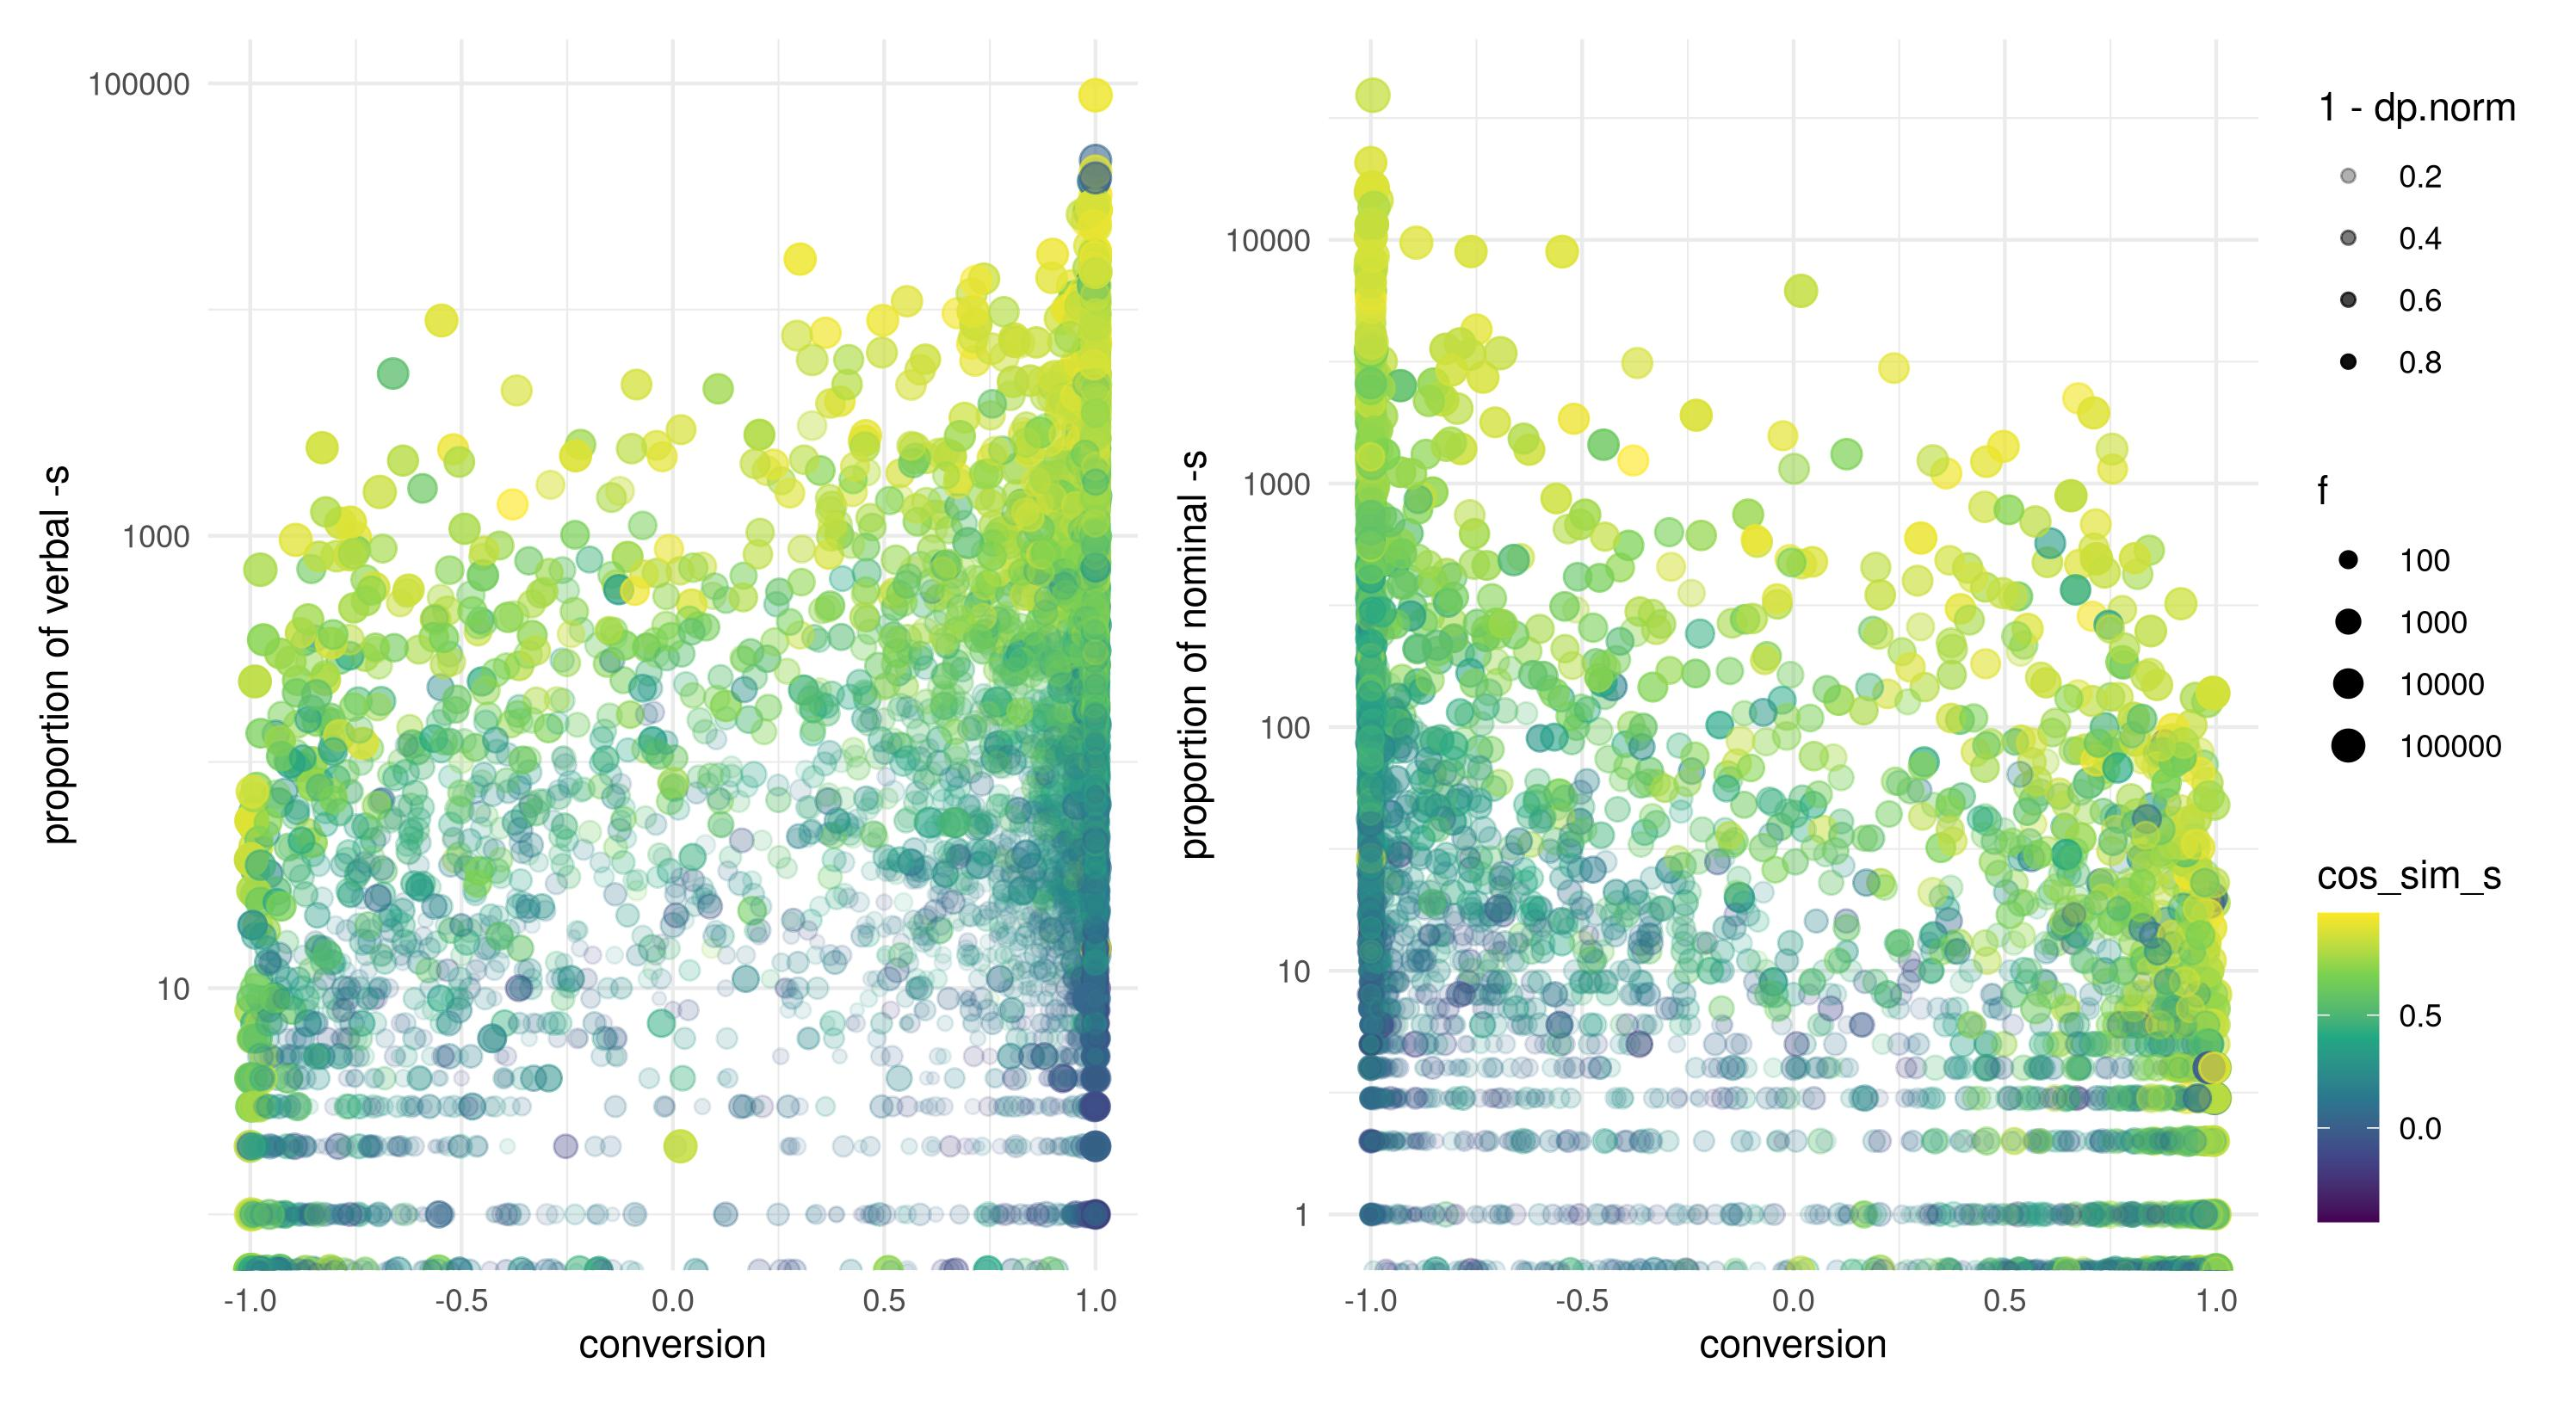
\includegraphics[width=\textwidth]{figures/s_continuum.jpg}
   \caption{Compound ratio of noun/verb POS tags against occurrences of *-s*}
   \label{s_continuum}
\end{figure}

The color shade in figure \ref{s_continuum} shows that the cosine
similarity between base and inflected form appears to be correlated with
a higher frequency of inflected forms. Part of the reason is that it is
weakly correlated with frequency. The variability lies in the fact that
some degree inflection, especially for plural \emph{-s}, might change
the use context considerably, and in extreme cases, be indicative of
highly conventionalized uses. Consider the following pairs:

\begin{enumerate}
\def\labelenumi{(\arabic{enumi})}
\setcounter{enumi}{4}
\tightlist
\item
  people, peoples (cosine similarity: \(0.54\))
\item
  world, worlds (cosine similarity: \(0.55\))
\item
  absence, absences (cosine similarity: \(0.55\))
\end{enumerate}

Compared to:

\begin{enumerate}
\def\labelenumi{(\arabic{enumi})}
\setcounter{enumi}{7}
\tightlist
\item
  word, words (cosine similarity: \(0.90\))
\item
  year, years (cosine similarity: \(0.92\))
\item
  suit, suits (cosine similarity: \(0.92\))
\end{enumerate}

In 5 to 7, the most common singular is semantically wildly different
from the most common plural use, while in 8 to 10 there is no
substantial change in meaning, not only between the singular and plural,
but also across the different polysemes/homonyms of the pairs.

Even though the measure is correlated with frequency, it shows little
correlation with the other measures listed above, except for
\(DP.norm\).

\hypertarget{analys}{%
\section{Analysis}\label{analys}}

\hypertarget{modeling-inflection-ratio}{%
\subsection{Modeling inflection ratio}\label{modeling-inflection-ratio}}

In the following sections, three different regression models will be
presented. Their purpose is mostly a first exploration of the
above-mentioned measures and their influence on inflection across the
verb-noun continuum. The relationship between the variables can be
expected to be non-monotonic and non-linear. To allow for the necessary
flexibility in the distribution and fit, the model framework chosen is
GAMLSS (\protect\hyperlink{ref-gamlss}{Rigby \& Stasinopoulos 2005}). It
is a semi-parametric approach that allows to fit a wide variety of
distributions, and combine linear terms with smoothed terms. The models
were created with the R package \emph{gamlss}
(\protect\hyperlink{ref-stasinopoulos17}{Stasinopoulos et al. 2017}).

The independent variable to be modeled was chosen to be the ratio of
inflected forms relative to all occurrences of a lemma that were tagged
as the compatible word class. Human perception has been found to be more
sensitive to proportional changes of stimuli rather than absolute ones
(cf. \protect\hyperlink{ref-kromer03}{Kromer 2003}). This makes counts
of inflected forms an inherently upper-bounded, compositional
phenomenon. The possible values can range from 0 to 1 inclusively.
Therefore, the distribution chosen to be fitted was a zero-one-inflated
beta distribution (\protect\hyperlink{ref-ospina+ferrari12}{Ospina \&
Ferrari 2012}; \protect\hyperlink{ref-rigby19}{Rigby et al. 2019}). Raw
counts of \emph{-s} could not be successfully modeled directly using
Poisson or negative (beta-)binomial regression, which led to highly
problematic model properties, and a very poor model fit, or outright
failure of the algorithm altogether.

Plain, relative or log frequencies did not improve the models, and
exhibited inferior performance compared to all other metrics. In fact,
model diagnostics became much worse in some cases. Possible reasons are
the problematic distributional properties of word frequencies, and low
frequency noise. Furthermore, frequency influences every of the
remaining metrics, so it is in a sense heavily encoded there. Therefore,
it was discarded in the final models presented here. \(DP.norm\) behaved
in a very similar way, which is not surprising since it correlates
strongly with frequency. Furthermore, it also correlates moderately with
the other measures, making it a kind of in-between measure. It was also
removed from the final models.

The above-mentioned measures, \(DWG\), \(DP.norm\) (ch.~\ref{disp}),
\(alpha_{1}\) for both left and right neighbors (ch.~\ref{hapax}), and
the conversion ratio introduced in (ch.~\ref{conv_measure}) where
finally picked as predictors. The first regression model attempts to
describe verbal uses of \emph{-s} based on parts-of-speech tagging (POS)
tagging. The second and third model repeat the same procedure for
nominal \emph{-s} and \emph{-ed}, both as past tense and past
participle.

\hypertarget{data}{%
\subsection{Data}\label{data}}

The data used to train the models was taken from the traditional BNC
(\protect\hyperlink{ref-bnc}{The British National Corpus 2007}). The
basic unit of analysis is lemmatized tokens, in combination with the
CLAWS POS tags. It has to be noted that conversion is not necessarily
restricted to single word units, but also possible for multi-word units
or entire phrases, in the same way that such units can be lexicalized
and stored as a whole. To keep the complexity of this study at a
manageable level, only lexemes represented by individual words are
considered. All metrics were calculated on all occurrences of a lemma
rather than the tuples of lemma and POS tag as it is typically done.
Like that, it is possible to capture a wider range of statistics per
item, while also minimizing any a priori categorization of items,
acknowledging the fact that lexical items in English are rather
flexible. The default assumption is that sameness in form has a strong
potential for lexical association between different uses. Of course,
this assumption is considerably weakened in the case of homographs. A
reliable method to annotate homographs, therefore, would be desirable.

Deverbal adjectives were filtered out based on POS tagging. Since the
measures used as dependent and independent variables are all inherently
ratio based, they are undefined at 0 occurrences of their significant
category. Therefore, the dataset had to be split into two separate
training sets, each with lemmas that occurred at least once as a verb
(for the verbal \emph{-s} and \emph{-ed} models), or once as a noun (for
the nominal \emph{-s} models). This explains the difference in sample
sizes (cf.~\ref{summaries}). A heuristic cut-off point of 50 occurrences
was chosen since all metrics are increasingly subject to quantization
effects and become rather unstable in lower frequency bands. Finally,
proper names were commonly mistagged as verbs in the datasets, causing
heavy tails in the residuals, and therefore excluded from the final
analysis.

\hypertarget{model-fit}{%
\subsection{Model fit}\label{model-fit}}

Table \ref{fit} shows the statistics for the residual distribution Means
and variances are very close to the desired values. The model for verbal
\emph{-s} also shows a heavy right tail, which is caused by a high
amount of extreme values. Arguably, this is not unusual for language
data, and might be related to the sample size. All models show some
degree of skew. An inherent property of the dataset is a potential for
multi-modality since the basic unit of analysis is lemmas. Clustering
techniques or fitting model mixes might be strategies for improvement,
without making arbitrary assumptions on lexical classes and creating
cut-off points, e.g.~for dominantly nominal vs.~dominantly verbal
lexemes.

\begin{longtable}[]{@{}lrrr@{}}
\caption{\label{fit}Statistics for residuals and fit of the three GAMLSS
models}\tabularnewline
\toprule
Metric & verbal -s & nominal -s & -ed \\
\midrule
\endfirsthead
\toprule
Metric & verbal -s & nominal -s & -ed \\
\midrule
\endhead
mean & -0.0382 & -0.0361 & 0.0261 \\
variance & 0.9816 & 0.9227 & 0.9043 \\
coef. of skewness & 0.5567 & 0.4772 & -0.2103 \\
coef. of kurtosis & 5.7153 & 3.1176 & 3.6533 \\
Filliben correlation coefficient & 0.9894 & 0.9916 & 0.9955 \\
pseudo R² & 0.6532 & 0.3914 & 0.3836 \\
\bottomrule
\end{longtable}

The overall deviance explained by the models is rather high for the
verbal \emph{-s} model and medium for the other two models. There is
much more variation on the nominal side of the spectrum, hence more
variation when it comes to plural \emph{-s}, which is also the most
frequent inflection in comparison. However, the predictions of the model
have to be taken with a grain of salt, since the distributional
properties of the data could not be fitted perfectly, resulting in
skewed residuals. Some potential factors could be the non-randomness of
the data, strong systematic noise, such as homography, and potential
unaccounted multimodality, e.g.~caused by other word classes.
Nevertheless, the applied dispersion and specificity measures allowed to
improve the fit drastically, and show promise for future improvements.

The full summary of the models including estimates, p-values and
confidence intervals for every coefficient can be found in the appendix,
ch.~\ref{summaries}, residual plots in ch.~\ref{diagnostics}.

\hypertarget{influence-of-conversion-on-nominal-and-verbal--s-vs--ed}{%
\subsection{\texorpdfstring{Influence of conversion on nominal and
verbal \emph{-s} vs
\emph{-ed}}{Influence of conversion on nominal and verbal -s vs -ed}}\label{influence-of-conversion-on-nominal-and-verbal--s-vs--ed}}

\begin{figure}[t!]
    \centering
    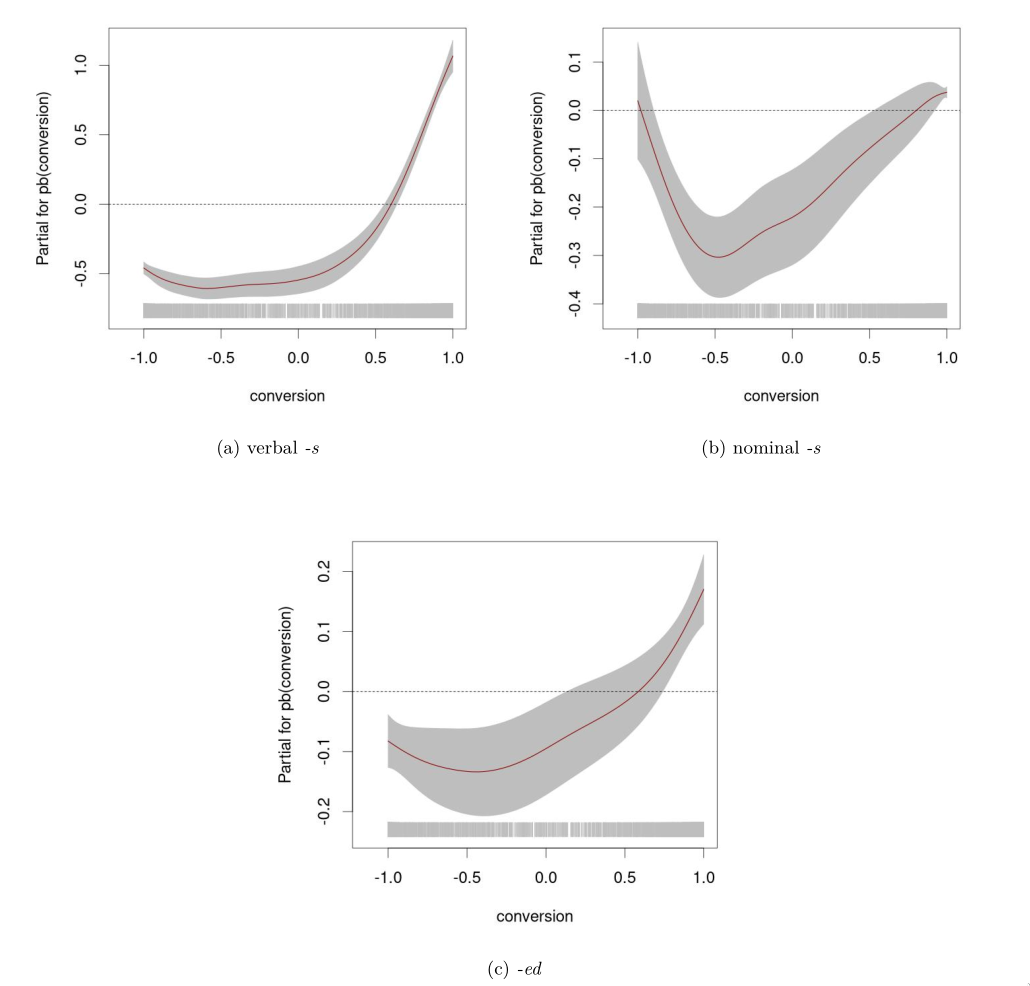
\includegraphics[width=\textwidth]{figures/docx_subfigures_1.png}
    \caption{Model estimates for conversion compared across the three models}
    \label{conv_pair}
\end{figure}

Figure \ref{conv_pair} shows a side by side comparison of the estimates
for conversion. The effect of conversion on nominal \emph{-s} follows a
distinct U-shape with both ends of the continuum having little to no
effect. Figure \ref{conv_pair}b shows a less pronounced U-shape, and a
much larger positive effect on the nominal side of the spectrum. In both
cases, there is a depression towards the middle of the continuum rather
than a simple monotonic relationship.

In comparison, the influence of conversion on \emph{-ed} is similar, but
much smaller and prone to more uncertainty as can be seen in figure
\ref{conv_pair}c.

\hypertarget{influence-of-dispersion-and-fixedness-in-context}{%
\subsection{Influence of dispersion and fixedness in
context}\label{influence-of-dispersion-and-fixedness-in-context}}

\begin{figure}[t!]
    \centering
    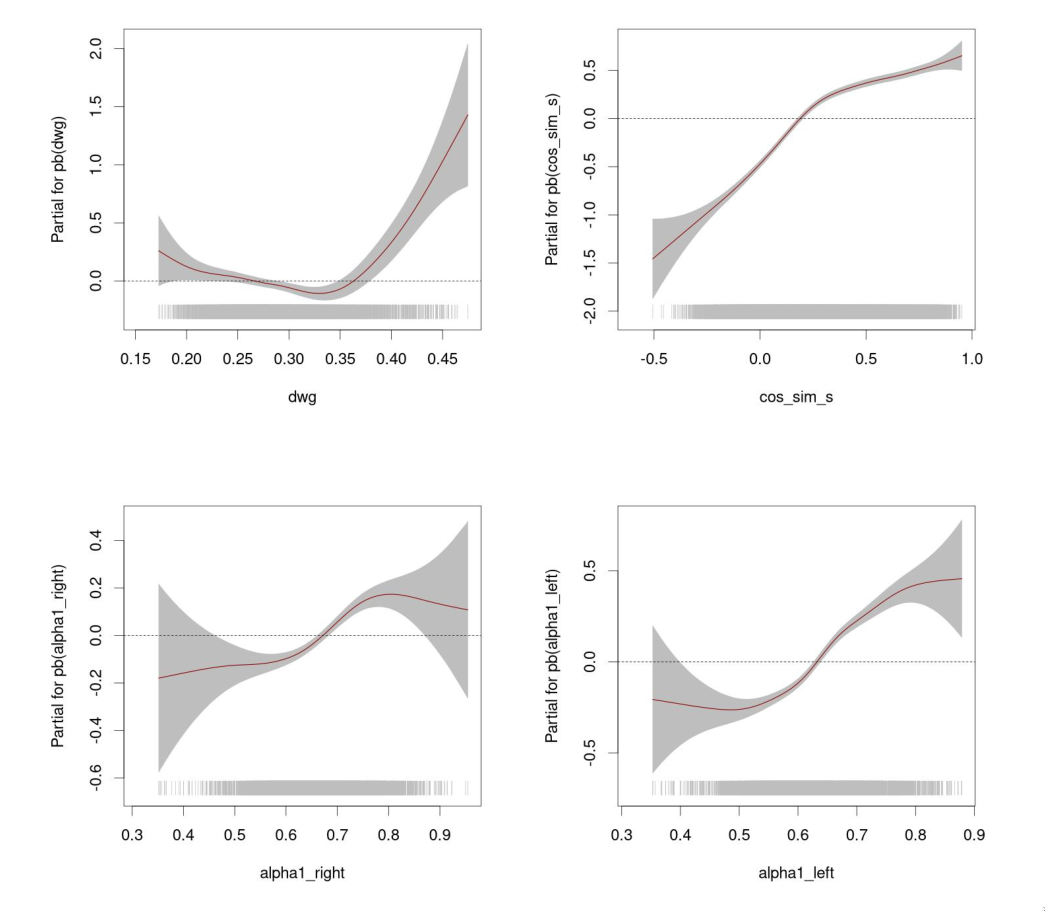
\includegraphics[width=\textwidth]{figures/docx_subfigures_2.png}
    \caption{Model estimates for conversion compared across the three models}
    \label{other_coefs_verb}
\end{figure}

Figure \ref{other_coefs_verb} shows the remaining coefficients for the
verbal \emph{-s} model.\footnote{When only one set of graphs is shown,
  the patterns depicted are roughly representative of those observed for
  the other two models unless further discussed.}

The effect of \(DWG\) was only significant in the model for nominal
\emph{-s} (see. section \ref{summaries}). There, it showed the expected
effect: a sharp increase of probability for inflection at high values.
Aside from that, controlling for \(DWG\) did improve the distribution of
residuals, and \(DWG\) had a significant and comparatively large effect
on the scale parameter in the verbal \emph{-s} model, indicating that it
could successfully account for some of the heteroscedasticity in the
distribution. The variation is higher in both extreme ends of the
measure. Interestingly, very highly dispersed lexemes show the most
variable behavior.

The boundedness to left- and right-hand-side tokens measured by
\(alpha_{1}\) shows a slightly positive effect for extremely flexible
lemmas, and a negative one for extremely inflexible ones. This pattern
holds across all models and is only subject to larger fluctuations at
the extreme ends. The largest slope can be observed in the left context
in the model for nominal \emph{-s} and the right context of verbal
\emph{-s} (cf.~\ref{summaries}). In the case of nouns, the left context
is where immediate morpho-syntactic markers occur, such as determiners.
This pattern could be an indication that inflected cases of conversion
are morpho-syntactically more restricted.

Finally, the cosine similarities from the GloVe embeddings show the most
distinct positive slope. A similarity in lexical co-occurrence patterns
between the base and its inflected form is correlated with a higher
proportion of occurrences of the inflectional form.

\hypertarget{zero-components-of-the-model}{%
\subsection{Zero components of the
model}\label{zero-components-of-the-model}}

\begin{figure}[t!]
    \centering
    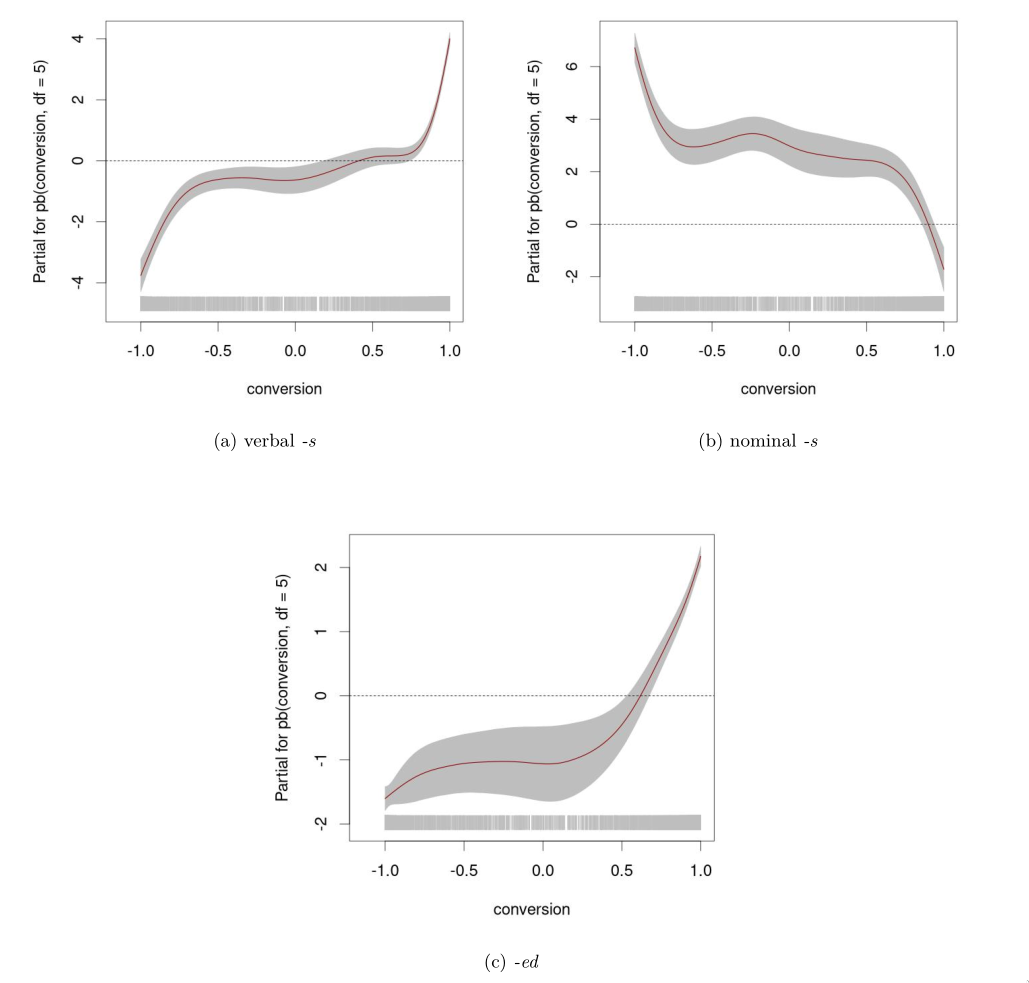
\includegraphics[width=\textwidth]{figures/docx_subfigures_3.png}
    \caption{Model estimates for conversion compared across the three models}
    \label{zero}
\end{figure}

Inflection is not semantically or functionally viable for all lexemes,
therefore there is a high amount of items that never occur inflected. As
compound models, the coefficients have different values for this zero
part of the distribution. Figure \ref{zero} shows the influence of
conversion and cosine similarity on the probability that a lexeme has an
inflection ratio of 0. The end points show a consistently high/low
influence towards the respective parts of the continuum. Pure verbs and
pure nouns have the lowest probability to stay uninflected when
occurring in their own word class, and high probabilities when rarely
converted. This drastically changes as long as there is some degree of
conversion.

The 1 components of the models were mostly inconclusive, and therefore
not visualized here. The reason for that lies in the extremely low
amount of items that were always inflected. Most of these items had
extreme values due to tagging or lemmatization errors. The few
legitimate observations had very low frequencies. For nominal \emph{-s},
pluralia tantum are a candidate category that has the potential to form
a cluster, but either it is not a productive category or the sample size
was just too low or the data too noisy to really see it. Furthermore,
even most pluralia tantum will eventually be analogically backformed or
otherwise used in a singular form at least once given a sufficiently
large sample size. Theoretically, verbal \emph{-s} has no plausible
category analogous with pluralia tantum, neither does \emph{-ed}.
Dropping the 1-inflated component and using a correction for ratios
equal to 1 appears to be a valid alternative strategy this type of
model.

\hypertarget{disc}{%
\section{Discussion}\label{disc}}

Modeling the proportion of \emph{-s} occurrences showed a generally
negative effect for items that are word class ambiguous. The probability
to occur with inflection sharply decreases towards the ``uncanny
valley'' of conversion. This decrease is more pronounced at the nominal
side of the continuum. Interestingly, however, the probability for
inflection seems to rise again towards the opposite side for all three
inflections. In the case of verb-noun conversion, this means that
inflectional marking is more common than expected for verbs that are not
too used as nouns, therefore, more strongly entrenched as verbs than
their more flexible counterparts toward the middle of the continuum. The
same can be said about the noun-verb conversion. The absence of
additional morphological cues might contribute to the difficulty in
processing. This is somewhat counter-balanced by higher inflection
ratios for very flexible collocates indicated by a positive effect of
the \(alpha_{1}\) and \(DWG\) values, i.e.~higher inflection ratio with
highly flexible, and well-dispersed uses.

Morever, a distinct U-shape can be observed for the effect of conversion
on nominal \emph{-s}. This suggests that verbs are as likely to be
pluralized when they are ad-hoc conversions or have rather rare nominal
homonyms/polysemes. The U-shape is less pronounced but noticeable in the
other models. It is possible that the missing entrenchment as
nominal/verbal lexeme, which potentially makes inflection a bit more
awkward, is counter-acted by other patterns. Additionally, the
probability that items never occur with the \emph{-s} suffix of their
respective dominant word class was shown to drastically decrease already
at rather low proportions of conversion. The lack of morphological
marking for word classes was expected to require additional
morpho-syntactical marking if the word class association is blurred,
since additional marking can increase the ease of processing. The
results, however, suggest that other distributional properties play a
much larger role.

\hypertarget{conc}{%
\section{Conclusion and Outlook}\label{conc}}

This study analyzed the underlying distribution of inflectional suffixes
across the verb-noun continuum, in order to trace effects of word class
ambiguity. There is a lot of structure in corpus data, and the
multivariate approach presented here shows a high potential for
identifying trends otherwise drowned by noisy data or covered by highly
skewed overlapping distributions. Additionally, understanding
morphological data as proportional, rather than count data, allows for
intuitive and conceptually interesting interpretations. The observations
in the corpus data are in line with previous research in phonetics and
neurolinguistic.

Measures of lexical fixedness/productivity more sophisticated than the
proposed fixed-window hapax ratio are also desirable, especially to
capture constructions, constructional idioms and other semi-fixed
structures. In fact, careful application and improvements on the entire
stack of corpus analysis are required, all the way from tokenization,
over lemmatization, to POS tagging. In future studies, customized
procedures have to be considered that are able to de-noise the
information required for a problem like ambiguity, rather than relying
on premade one-size-fits-all solutions. This comes at a considerable
computation effort but is becoming more and more feasible with modern
hardware and/or distributed systems.

Word embeddings, dispersion measures and association statistics show
that individual word statistics work best when taking into account the
entire corpus. Word embeddings and more recent transformer networks like
BERT may provide an interesting route for further studies in ambiguity
(e.g. \protect\hyperlink{ref-beekhuizen_et_al21}{Beekhuizen, Armstrong
\& Stevenson 2021}; \protect\hyperlink{ref-du_et_al19}{Du, Qi \& Sun
2019}; \protect\hyperlink{ref-wiedemann19}{Wiedemann et al. 2019}).
Clustering techniques can be used to detect homonymy
(\protect\hyperlink{ref-lee21}{Lee 2021}), which could be used for
corpus annotation as an addition to or replacement of classical
lemmatization. If proven robust and carefully applied, this could
potentially lead to further decreases in noise. The recent successes of
word2vec, BERT etc. in practical application are promising for the use
in a more descriptive application. They can provide another angle on
co-occurrence statistics, and were only sparsely used in this study
since there has been little systematic application in corpus linguistics
prior to this point. The mentioned techniques can be further enriched by
including more contextual and ``world knowledge'' information, such as
images (e.g. \protect\hyperlink{ref-kottur16}{Kottur et al. 2016};
\protect\hyperlink{ref-shahmohammadi21}{Shahmohammadi, Lensch \& Baayen
2021}). For the time being, more well-understood dispersion measures,
measures of productivity and simple context embeddings can still provide
tools to further test where real ambiguity exists and how it affects the
system of language.

\newpage

\hypertarget{appendix}{%
\section{Appendix}\label{appendix}}

\hypertarget{summaries}{%
\subsection{Model summaries}\label{summaries}}

\hypertarget{verbal--s}{%
\subsubsection{\texorpdfstring{Verbal
\emph{-s}}{Verbal -s}}\label{verbal--s}}

\small

\begin{verbatim}
# Fixed Effects

Parameter    | Coefficient |   SE |         95% CI | t(5810.18) |      p
------------------------------------------------------------------------
(Intercept)  |       -4.79 | 0.24 | [-5.26, -4.33] |     -20.20 | < .001
conversion   |        0.56 | 0.02 | [ 0.51,  0.60] |      24.16 | < .001
dwg          |        0.07 | 0.37 | [-0.66,  0.81] |       0.20 | 0.841 
cos_sim_s    |        0.90 | 0.05 | [ 0.79,  1.00] |      16.73 | < .001
alpha1_right |        1.89 | 0.23 | [ 1.45,  2.34] |       8.28 | < .001
alpha1_left  |        1.47 | 0.20 | [ 1.09,  1.86] |       7.53 | < .001

# Sigma

Parameter              | Coefficient |   SE |         95% CI | t(5810.18) |      p
----------------------------------------------------------------------------------
(Intercept)            |       -3.15 | 0.24 | [-3.62, -2.68] |     -13.25 | < .001
pb(conversion, df = 5) |        0.64 | 0.02 | [ 0.60,  0.68] |      30.04 | < .001
dwg                    |        2.05 | 0.36 | [ 1.34,  2.76] |       5.66 | < .001
alpha1_right           |        1.16 | 0.24 | [ 0.69,  1.62] |       4.86 | < .001
alpha1_left            |        1.24 | 0.21 | [ 0.84,  1.65] |       5.97 | < .001
cos_sim_s              |        0.27 | 0.05 | [ 0.16,  0.37] |       4.90 | < .001

# Nu

Parameter              | Coefficient |   SE |         95% CI | t(5810.18) |      p
----------------------------------------------------------------------------------
(Intercept)            |       -2.47 | 0.73 | [-3.89, -1.05] |      -3.41 | < .001
pb(conversion, df = 5) |        2.85 | 0.09 | [ 2.67,  3.03] |      31.07 | < .001
dwg                    |       -0.02 | 0.96 | [-1.91,  1.87] |      -0.02 | 0.982 
alpha1_right           |        0.47 | 0.72 | [-0.93,  1.88] |       0.66 | 0.511 
alpha1_left            |        1.39 | 0.69 | [ 0.03,  2.74] |       2.01 | 0.045 
cos_sim_s              |       -2.16 | 0.17 | [-2.49, -1.83] |     -12.84 | < .001

# Tau

Parameter              | Coefficient |   SE |          95% CI | t(5810.18) |      p
-----------------------------------------------------------------------------------
(Intercept)            |      -14.11 | 3.06 | [-20.10, -8.12] |      -4.62 | < .001
pb(conversion, df = 5) |        4.92 | 2.01 | [  0.98,  8.85] |       2.45 | 0.014 
dwg                    |       -1.83 | 2.52 | [ -6.77,  3.10] |      -0.73 | 0.467 
alpha1_right           |        1.96 | 1.88 | [ -1.73,  5.66] |       1.04 | 0.298 
alpha1_left            |        9.45 | 2.68 | [  4.20, 14.71] |       3.52 | < .001
cos_sim_s              |       -2.13 | 0.64 | [ -3.38, -0.88] |      -3.33 | < .001
\end{verbatim}

\begin{verbatim}
------------------------------------------------------------------ 
 No. of observations in the fit:  5923  
 Degrees of Freedom for the fit:  112.8151 
       Residual Deg. of Freedom:  5810.185  
                       at cycle:  30  
   
 Global Deviance:     -9669.721  
             AIC:     -9444.091  
             SBC:     -8689.741  
 ------------------------------------------------------------------ 
\end{verbatim}

\normalsize
\newpage

\hypertarget{nominal--s}{%
\subsubsection{\texorpdfstring{Nominal
\emph{-s}}{Nominal -s}}\label{nominal--s}}

\small

\begin{verbatim}
# Fixed Effects

Parameter    | Coefficient |   SE |         95% CI | t(12117.43) |      p
-------------------------------------------------------------------------
(Intercept)  |       -4.61 | 0.15 | [-4.91, -4.31] |      -29.87 | < .001
conversion   |        0.12 | 0.02 | [ 0.08,  0.17] |        6.11 | < .001
dwg          |        1.35 | 0.20 | [ 0.96,  1.73] |        6.77 | < .001
cos_sim_s    |        1.37 | 0.04 | [ 1.30,  1.45] |       36.57 | < .001
alpha1_right |        1.58 | 0.16 | [ 1.28,  1.89] |       10.22 | < .001
alpha1_left  |        2.68 | 0.15 | [ 2.39,  2.97] |       18.36 | < .001

# Sigma

Parameter              | Coefficient |   SE |         95% CI | t(12117.43) |      p
-----------------------------------------------------------------------------------
(Intercept)            |        0.55 | 0.14 | [ 0.28,  0.83] |        3.91 | < .001
pb(conversion, df = 5) |        0.03 | 0.02 | [-0.01,  0.07] |        1.45 | 0.146 
dwg                    |        0.24 | 0.18 | [-0.12,  0.60] |        1.31 | 0.190 
alpha1_right           |       -0.83 | 0.14 | [-1.11, -0.55] |       -5.85 | < .001
alpha1_left            |        0.09 | 0.13 | [-0.17,  0.36] |        0.70 | 0.485 
cos_sim_s              |       -0.91 | 0.04 | [-0.98, -0.84] |      -25.15 | < .001

# Nu

Parameter              | Coefficient |   SE |         95% CI | t(12117.43) |      p
-----------------------------------------------------------------------------------
(Intercept)            |       -1.06 | 1.28 | [-3.57,  1.45] |       -0.83 | 0.408 
pb(conversion, df = 5) |       -2.96 | 0.16 | [-3.27, -2.66] |      -18.98 | < .001
dwg                    |       -5.05 | 2.05 | [-9.06, -1.04] |       -2.47 | 0.014 
alpha1_right           |       -2.72 | 1.21 | [-5.10, -0.35] |       -2.25 | 0.025 
alpha1_left            |        1.24 | 0.97 | [-0.66,  3.15] |        1.28 | 0.201 
cos_sim_s              |       -1.90 | 0.31 | [-2.50, -1.30] |       -6.19 | < .001

# Tau

Parameter              | Coefficient |   SE |          95% CI | t(12117.43) |      p
------------------------------------------------------------------------------------
(Intercept)            |       -8.92 | 1.40 | [-11.67, -6.17] |       -6.36 | < .001
pb(conversion, df = 5) |       -1.00 | 0.12 | [ -1.23, -0.77] |       -8.46 | < .001
dwg                    |        4.66 | 1.75 | [  1.24,  8.09] |        2.67 | 0.008 
alpha1_right           |       -0.47 | 1.35 | [ -3.12,  2.18] |       -0.35 | 0.726 
alpha1_left            |        5.64 | 1.30 | [  3.10,  8.18] |        4.35 | < .001
cos_sim_s              |       -1.06 | 0.40 | [ -1.84, -0.27] |       -2.63 | 0.009 
\end{verbatim}

\begin{verbatim}
------------------------------------------------------------------ 
 No. of observations in the fit:  12198  
 Degrees of Freedom for the fit:  80.57188 
       Residual Deg. of Freedom:  12117.43  
                       at cycle:  14  
   
 Global Deviance:     -10043.74  
             AIC:     -9882.6  
             SBC:     -9285.641  
 ------------------------------------------------------------------ 
\end{verbatim}

\normalsize
\newpage

\hypertarget{ed}{%
\subsubsection{\texorpdfstring{\emph{-ed}}{-ed}}\label{ed}}

\small

\begin{verbatim}
# Fixed Effects

Parameter    | Coefficient |   SE |         95% CI | t(5861.88) |      p
------------------------------------------------------------------------
(Intercept)  |       -1.60 | 0.24 | [-2.08, -1.12] |      -6.57 | < .001
conversion   |        0.11 | 0.02 | [ 0.07,  0.14] |       5.41 | < .001
dwg          |        0.16 | 0.39 | [-0.59,  0.92] |       0.42 | 0.673 
alpha1_right |        1.85 | 0.23 | [ 1.39,  2.31] |       7.92 | < .001
alpha1_left  |        0.16 | 0.20 | [-0.24,  0.56] |       0.79 | 0.429 

# Sigma

Parameter              | Coefficient |   SE |         95% CI | t(5861.88) |      p
----------------------------------------------------------------------------------
(Intercept)            |        1.09 | 0.23 | [ 0.65,  1.54] |       4.79 | < .001
pb(conversion, df = 5) |        0.02 | 0.02 | [-0.02,  0.06] |       1.04 | 0.301 
dwg                    |        0.14 | 0.37 | [-0.58,  0.85] |       0.37 | 0.709 
alpha1_right           |       -1.40 | 0.23 | [-1.84, -0.95] |      -6.10 | < .001
alpha1_left            |       -0.55 | 0.20 | [-0.96, -0.15] |      -2.70 | 0.007 

# Nu

Parameter              | Coefficient |   SE |          95% CI | t(5861.88) |      p
-----------------------------------------------------------------------------------
(Intercept)            |       -9.45 | 0.64 | [-10.71, -8.18] |     -14.65 | < .001
pb(conversion, df = 5) |        1.70 | 0.07 | [  1.58,  1.83] |      25.84 | < .001
dwg                    |        2.93 | 0.90 | [  1.15,  4.70] |       3.23 | 0.001 
alpha1_right           |        2.98 | 0.64 | [  1.73,  4.23] |       4.68 | < .001
alpha1_left            |        7.24 | 0.62 | [  6.03,  8.46] |      11.69 | < .001

# Tau

Parameter              | Coefficient |   SE |          95% CI | t(5861.88) |      p
-----------------------------------------------------------------------------------
(Intercept)            |      -10.75 | 1.09 | [-12.89, -8.62] |      -9.87 | < .001
pb(conversion, df = 5) |        3.49 | 0.37 | [  2.77,  4.22] |       9.44 | < .001
dwg                    |        1.81 | 1.49 | [ -1.11,  4.73] |       1.21 | 0.225 
alpha1_right           |        2.13 | 1.10 | [ -0.03,  4.29] |       1.93 | 0.054 
alpha1_left            |        6.14 | 1.08 | [  4.02,  8.27] |       5.67 | < .001
\end{verbatim}

\begin{verbatim}
------------------------------------------------------------------ 
 No. of observations in the fit:  5923  
 Degrees of Freedom for the fit:  61.11825 
       Residual Deg. of Freedom:  5861.882  
                       at cycle:  8  
   
 Global Deviance:     4316.905  
             AIC:     4439.142  
             SBC:     4847.815  
 ------------------------------------------------------------------ 
\end{verbatim}

\normalsize
\newpage

\hypertarget{nomenclature}{%
\subsection{Nomenclature}\label{nomenclature}}

All models are zero-one-inflated beta regressions with the proportion of
inflection as dependent variable. \(Sigma\) coefficients represent the
scale parameter of the distribution, \(Nu\) and \(Tau\) represent the 0
and 1 component respectively. All coefficients were fitted using
p-splines. Non-fixed effects were set to \(df = 5\) to control for
overfitting. The mean and scale parameter use the pre-specified logit
link function. \(Nu\) and \(Tau\) have log link functions.

\hypertarget{diagnostics}{%
\subsection{Residual plots}\label{diagnostics}}

\begin{figure}
     \centering
     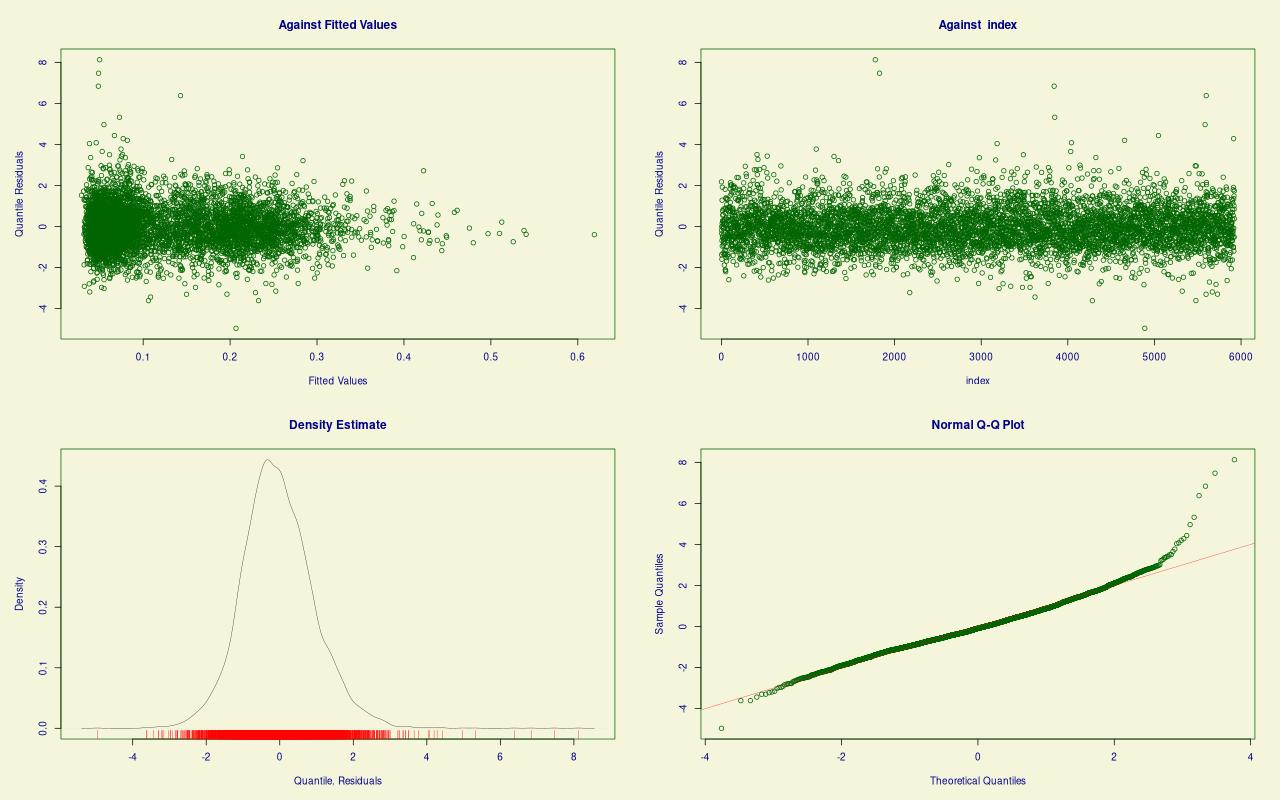
\includegraphics[width=\textwidth]{figures/m_verb_diagnostic.jpg}
     \caption{Diagnostics for beta inflated GAMLSS model predicting proportions of verbal \textit{-s}}
     \label{verb_diagnostics}
\end{figure}

\begin{figure}
     \centering
     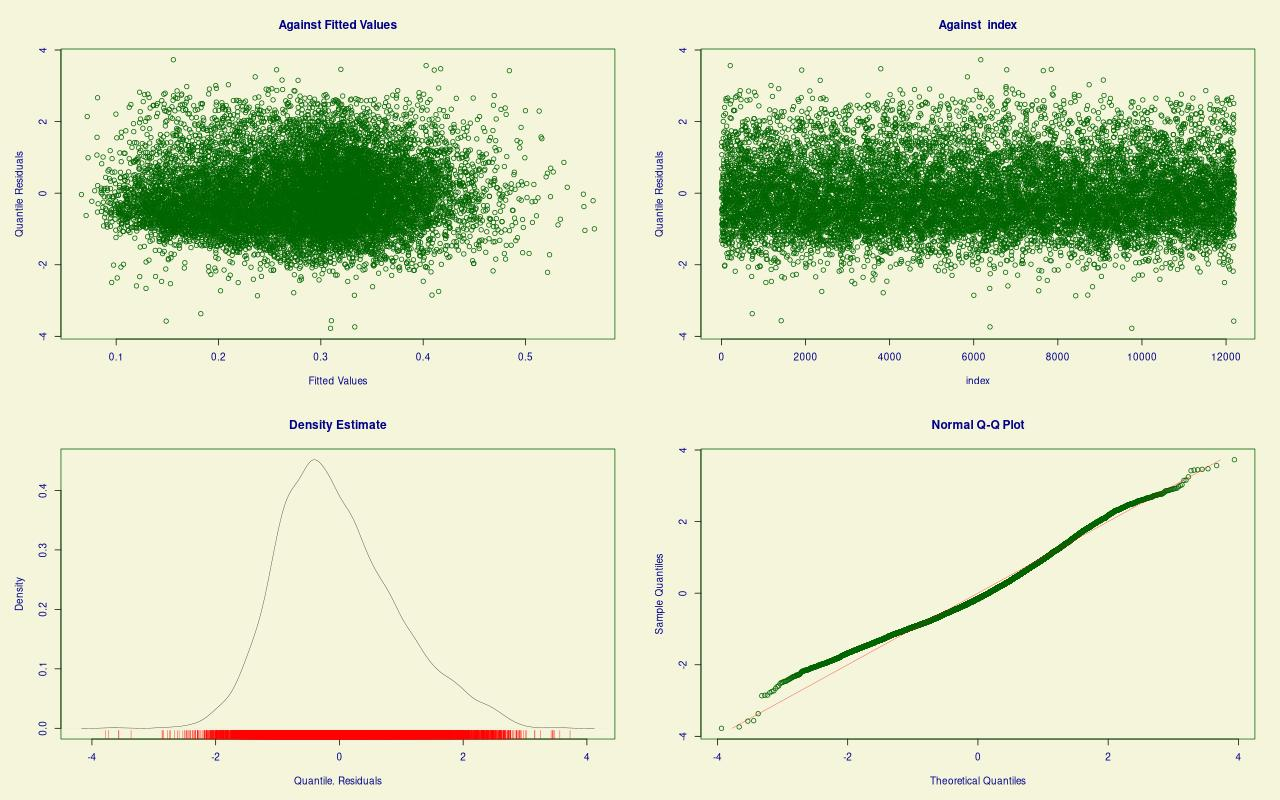
\includegraphics[width=\textwidth]{figures/m_noun_diagnostic.jpg}
     \caption{Diagnostics for beta inflated GAMLSS model predicting proportions of nominal \textit{-s}}
     \label{noun_diagnostics}
\end{figure}

\begin{figure}
     \centering
     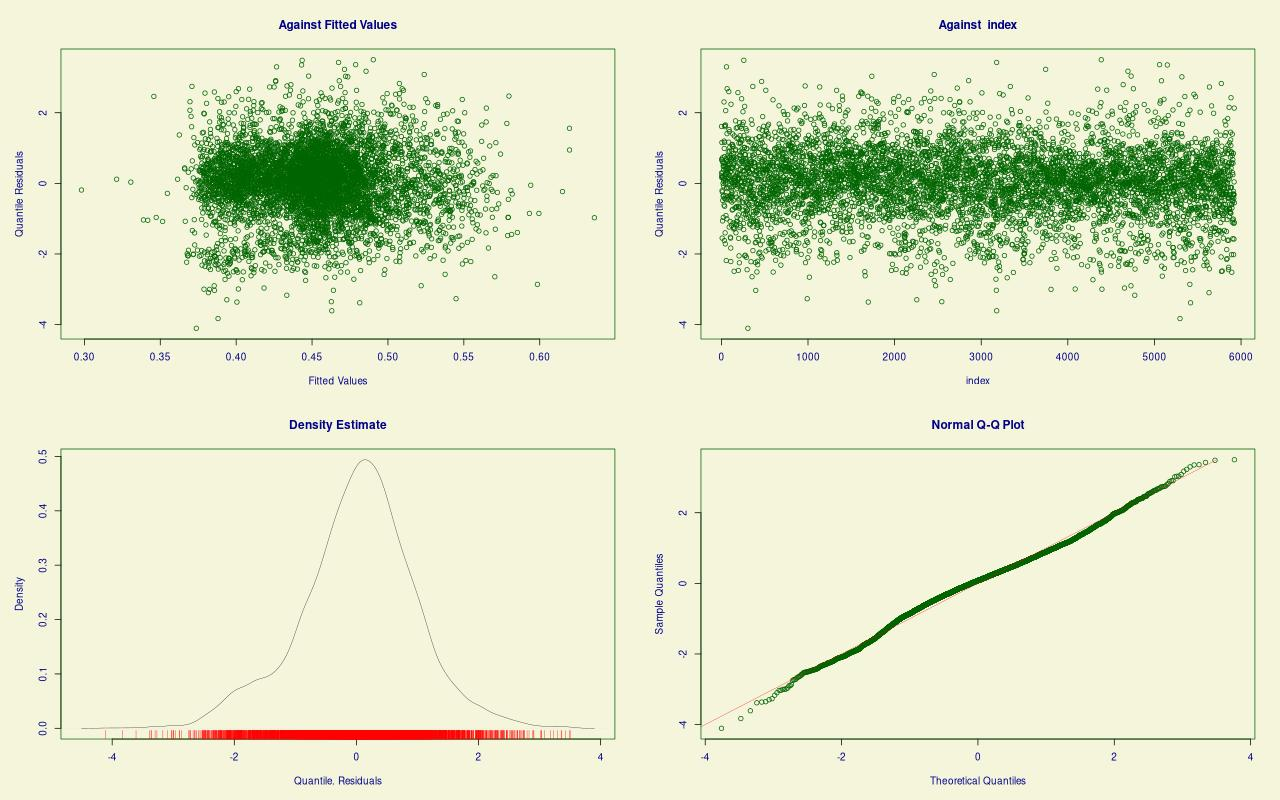
\includegraphics[width=\textwidth]{figures/m_ed_diagnostic.jpg}
     \caption{Diagnostics for beta inflated GAMLSS model predicting proportions of \textit{-ed}}
     \label{ed_diagnostics}
\end{figure}

\newpage

\hypertarget{bibliography}{%
\section{Bibliography}\label{bibliography}}

\hypertarget{refs}{}
\begin{CSLReferences}{1}{0}
\leavevmode\vadjust pre{\hypertarget{ref-beekhuizen_et_al21}{}}%
Beekhuizen, Barend, Blair C. Armstrong \& Suzanne Stevenson. 2021.
Probing lexical ambiguity: Word vectors encode number and relatedness of
senses. \emph{Cognitive Science} 45(5). e12943.
\url{https://doi.org/10.1111/cogs.12943}.
\url{https://onlinelibrary.wiley.com/doi/abs/10.1111/cogs.12943}.

\leavevmode\vadjust pre{\hypertarget{ref-bultena_et_al13}{}}%
Bultena, Sybrine, Ton Dijkstra \& Janet G. van Hell. 2013. Cognate and
word class ambiguity effects in noun and verb processing. \emph{Language
and Cognitive Processes}. Routledge 28(9). 1350--1377.
\url{https://doi.org/10.1080/01690965.2012.718353}.

\leavevmode\vadjust pre{\hypertarget{ref-diessel16}{}}%
Diessel, Holger. 2016. Frequency and lexical specificity in grammar: A
critical review. In Heike Behrens \& Stefan Pfänder (eds.),
\emph{Experience counts: Frequency effects in language}, 209--238. De
Gruyter. \url{https://doi.org/10.1515/9783110346916-009}.

\leavevmode\vadjust pre{\hypertarget{ref-data.table}{}}%
Dowle, Matt \& Arun Srinivasan. 2021. \emph{Data.table: Extension of
`data.frame`}. \url{https://CRAN.R-project.org/package=data.table}.

\leavevmode\vadjust pre{\hypertarget{ref-du_et_al19}{}}%
Du, Jiaju, Fanchao Qi \& Maosong Sun. 2019. Using {BERT} for word sense
disambiguation. \emph{CoRR} abs/1909.08358.
\url{http://arxiv.org/abs/1909.08358}.

\leavevmode\vadjust pre{\hypertarget{ref-evert05}{}}%
Evert, Stefan. 2005. \emph{The statistics of word cooccurrences: Word
pairs and collocations}. Friedrich-Alexander-Universität
Erlangen-Nürnberg PhD thesis. \url{http://www.collocations.de/phd.html}.

\leavevmode\vadjust pre{\hypertarget{ref-cwb}{}}%
Evert, Stefan \& Andrew Hardie. 2011. Twenty-first century corpus
workbench: Updating a query architecture for the new millennium.
University of Birmingham.

\leavevmode\vadjust pre{\hypertarget{ref-federmeier_et_al00}{}}%
Federmeier, Kara D., Jessica B. Segal, Tania Lombrozo \& Marta Kutas.
2000. {Brain responses to nouns, verbs and class-ambiguous words in
context}. \emph{Brain} 123(12). 2552--2566.
\url{https://doi.org/10.1093/brain/123.12.2552}.
\url{https://doi.org/10.1093/brain/123.12.2552}.

\leavevmode\vadjust pre{\hypertarget{ref-gries21}{}}%
Gries, Stefan. 2021. A new approach to (key) keywords analysis: Using
frequency, and now also dispersion. \emph{Research in Corpus
Linguistics} 9(2). 1--33. \url{https://doi.org/10.32714/ricl.09.02.02}.

\leavevmode\vadjust pre{\hypertarget{ref-gries08}{}}%
Gries, Stefan Th. 2008. Dispersions and adjusted frequencies in corpora.
\emph{International journal of corpus linguistics}. John Benjamins
13(4). 403--437.

\leavevmode\vadjust pre{\hypertarget{ref-kottur16}{}}%
Kottur, Satwik, Ramakrishna Vedantam, José MF Moura \& Devi Parikh.
2016. Visual word2vec (vis-w2v): Learning visually grounded word
embeddings using abstract scenes. In \emph{Proceedings of the IEEE
conference on computer vision and pattern recognition}, 4985--4994.

\leavevmode\vadjust pre{\hypertarget{ref-kromer03}{}}%
Kromer, Victor. 2003. A usage measure based on psychophysical relations.
\emph{Journal of Quantitative Linguistics}. Taylor \& Francis 10(2).
177--186.

\leavevmode\vadjust pre{\hypertarget{ref-lee06}{}}%
Lee, Chia-lin \& Kara D. Federmeier. 2006. To mind the mind: An
event-related potential study of word class and semantic ambiguity.
\emph{Brain Research} 1081(1). 191--202.
\url{https://doi.org/doi.org/10.1016/j.brainres.2006.01.058}.
\url{https://www.sciencedirect.com/science/article/pii/S0006899306001727}.

\leavevmode\vadjust pre{\hypertarget{ref-lee+federmeier08}{}}%
Lee, Chia-lin \& Kara D. Federmeier. 2008. To watch, to see, and to
differ: An event-related potential study of concreteness effects as a
function of word class and lexical ambiguity. \emph{Brain and Language}
104(2). 145--158.
\url{https://doi.org/doi.org/10.1016/j.bandl.2007.06.002}.
\url{https://www.sciencedirect.com/science/article/pii/S0093934X07001174}.

\leavevmode\vadjust pre{\hypertarget{ref-lee21}{}}%
Lee, Younghoon. 2021. Systematic homonym detection and replacement based
on contextual word embedding. \emph{Neural Processing Letters} 53(1).
17--36. \url{https://doi.org/10.1007/s11063-020-10376-8}.

\leavevmode\vadjust pre{\hypertarget{ref-lijffijt+gries12}{}}%
Lijffijt, Jefrey \& Stefan Th Gries. 2012. Correction to stefan th.
Gries'{``dispersions and adjusted frequencies in corpora''}
international journal of corpus linguistics 13: 4 (2008), 403-437.
Citeseer.

\leavevmode\vadjust pre{\hypertarget{ref-ospina+ferrari12}{}}%
Ospina, Raydonal \& Silvia L. P. Ferrari. 2012. A general class of
zero-or-one inflated beta regression models. \emph{Computational
Statistics \& Data Analysis} 56(6). 1609--1623.
\url{https://doi.org/10.1016/j.csda.2011.10.005}.
\url{https://www.sciencedirect.com/science/article/pii/S0167947311003628}.

\leavevmode\vadjust pre{\hypertarget{ref-pennington14}{}}%
Pennington, Jeffrey, Richard Socher \& Christopher D Manning. 2014.
Glove: Global vectors for word representation. In \emph{Proceedings of
the 2014 conference on empirical methods in natural language processing
(EMNLP)}, 1532--1543.

\leavevmode\vadjust pre{\hypertarget{ref-piantadosi_et_al12}{}}%
Piantadosi, Steven T., Harry Tily \& Edward Gibson. 2012. The
communicative function of ambiguity in language. \emph{Cognition}
122(3). 280--291. \url{https://doi.org/10.1016/j.cognition.2011.10.004}.
\url{https://www.sciencedirect.com/science/article/pii/S0010027711002496}.

\leavevmode\vadjust pre{\hypertarget{ref-plag17}{}}%
Plag, Ingo, Julia Homann \& Gero Kunter. 2017. Homophony and morphology:
The acoustics of word-final s in english. \emph{Journal of Linguistics}.
Cambridge University Press 53(1). 181--216.

\leavevmode\vadjust pre{\hypertarget{ref-R_base}{}}%
R Core Team. 2021. \emph{R: A language and environment for statistical
computing}. Vienna, Austria: R Foundation for Statistical Computing.
\url{https://www.R-project.org/}.

\leavevmode\vadjust pre{\hypertarget{ref-gamlss}{}}%
Rigby, R. A. \& D. M. Stasinopoulos. 2005. Generalized additive models
for location, scale and shape, (with discussion). \emph{Applied
Statistics} 54.3. 507--554.

\leavevmode\vadjust pre{\hypertarget{ref-rigby19}{}}%
Rigby, Robert A, Mikis D Stasinopoulos, Gillian Z Heller \& Fernanda De
Bastiani. 2019. \emph{Distributions for modeling location, scale, and
shape: Using GAMLSS in r}. Chapman; Hall/CRC.

\leavevmode\vadjust pre{\hypertarget{ref-text2vec}{}}%
Selivanov, Dmitriy, Manuel Bickel \& Qing Wang. 2020. \emph{text2vec:
Modern text mining framework for r}.
\url{https://CRAN.R-project.org/package=text2vec}.

\leavevmode\vadjust pre{\hypertarget{ref-shahmohammadi21}{}}%
Shahmohammadi, Hassan, Hendrik Lensch \& R Harald Baayen. 2021. Learning
zero-shot multifaceted visually grounded word embeddings via multi-task
training. \emph{arXiv preprint arXiv:2104.07500}.

\leavevmode\vadjust pre{\hypertarget{ref-stasinopoulos18}{}}%
Stasinopoulos, Mikis D, Robert A Rigby \& Fernanda De Bastiani. 2018.
GAMLSS: A distributional regression approach. \emph{Statistical
Modelling}. SAGE Publications Sage India: New Delhi, India 18(3-4).
248--273.

\leavevmode\vadjust pre{\hypertarget{ref-stasinopoulos17}{}}%
Stasinopoulos, Mikis D, Robert A Rigby, Gillian Z Heller, Vlasios
Voudouris \& Fernanda De Bastiani. 2017. \emph{Flexible regression and
smoothing: Using GAMLSS in r}. CRC Press.

\leavevmode\vadjust pre{\hypertarget{ref-bnc}{}}%
The British National Corpus, version 3 (BNC XML Edition). 2007.
\url{http://www.natcorp.ox.ac.uk/}; Distributed by Bodleian Libraries,
University of Oxford, on behalf of the BNC Consortium.

\leavevmode\vadjust pre{\hypertarget{ref-tomaschek_et_al21}{}}%
Tomaschek, Fabian, Ingo Plag, Mirjam Ernestus \& R. Harald Baayen. 2021.
Phonetic effects of morphology and context: Modeling the duration of
word-final s in english with naïve discriminative learning.
\emph{Journal of Linguistics}. Cambridge University Press 57(1).
123--161. \url{https://doi.org/10.1017/S0022226719000203}.

\leavevmode\vadjust pre{\hypertarget{ref-tomaschek_et_al_18}{}}%
Tomaschek, Fabian, Benjamin V. Tucker, Matteo Fasiolo \& R. Harald
Baayen. 2018. Practice makes perfect: The consequences of lexical
proficiency for articulation: \emph{Linguistics Vanguard} 4(s2).
20170018. \url{https://doi.org/doi:10.1515/lingvan-2017-0018}.

\leavevmode\vadjust pre{\hypertarget{ref-trott+bergen20}{}}%
Trott, Sean \& Benjamin Bergen. 2020. Why do human languages have
homophones? \emph{Cognition} 205. 104449.
\url{https://doi.org/10.1016/j.cognition.2020.104449}.
\url{https://www.sciencedirect.com/science/article/pii/S0010027720302687}.

\leavevmode\vadjust pre{\hypertarget{ref-wasow15}{}}%
Wasow, Thomas. 2015. Ambiguity avoidance is overrated. In Susanne
Winkler (ed.), \emph{Ambiguity}, 29--48. De Gruyter.
\url{https://doi.org/10.1515/9783110403589-003}.

\leavevmode\vadjust pre{\hypertarget{ref-ggplot}{}}%
Wickham, Hadley. 2016. \emph{ggplot2: Elegant graphics for data
analysis}. Springer-Verlag New York.
\url{https://ggplot2.tidyverse.org}.

\leavevmode\vadjust pre{\hypertarget{ref-wiedemann19}{}}%
Wiedemann, Gregor, Steffen Remus, Avi Chawla \& Chris Biemann. 2019.
Does BERT make any sense? Interpretable word sense disambiguation with
contextualized embeddings. \emph{arXiv preprint arXiv:1909.10430}.

\leavevmode\vadjust pre{\hypertarget{ref-song_et_al13}{}}%
Yung Song, Jae, Katherine Demuth, Karen Evans \& Stefanie
Shattuck-Hufnagel. 2013. Durational cues to fricative codas in
2-year-olds' american english: Voicing and morphemic factors. \emph{The
Journal of the Acoustical Society of America}. Acoustical Society of
America 133(5). 2931--2946.

\leavevmode\vadjust pre{\hypertarget{ref-zimmermann20}{}}%
Zimmermann, Richard. 2020. Word growth dispersion---a single corpus part
measure of lexical dispersion. Paper presented at ICAME41 Heidelberg.
\url{https://www.youtube.com/watch?v=k8etOvRcF4c}.

\end{CSLReferences}

\end{document}
